\subsection{Regressione}
Immaginiamo di andare in laboratorio e di raccogliere i dati di un esperimento. Quello che si è soliti fare è disporre i dati su due colonne: una raccoglie le variabili indipendenti, l'altra quelle dipendenti, che solitamente indichiamo rispettivamente con $x$ e $y$. Supponiamo quindi di avere raccolto $n+1$ dati $(x_i,y_i)$ con $i=0,\ldots,n$. Di norma gli $x_i$ sono degli scalari, ma più raramente può capitare che siano delle $p$-uple, cioè degli elementi di $\mathbb{R}^p$. Tale situazione corrisponde al caso in cui la variabile dipendente $y_i$ (che in entrambi i casi è uno scalare) dipende da diverse variabili indipendenti. Ci limiteremo al primo caso.

Ciò che di solito si fa in laboratorio è supporre di conoscere la forma funzionale $f$ della dipendenza teorica tra $y$ e $x$. In generale tale forma dipenderà da diversi parametri che indichiamo in forma vettoriale con $\underline{a}$, il quale in generale sarà una $q$-upla:

$$y=f( \underline{x};\underline{a} )$$

Il primo problema che affrontiamo in laboratorio è quello di trovare i valori più probabili\footnote{Qui e nel seguito il prof usa il termine "the most likely". Non essendo sicuro sulla traduzione più adatta a volte ho tradotto a senso.} di tali parametri che interpolano tra i dati forniti.

\vspace{0.3cm}

\begin{minipage}{0.445\textwidth}
   \centering
   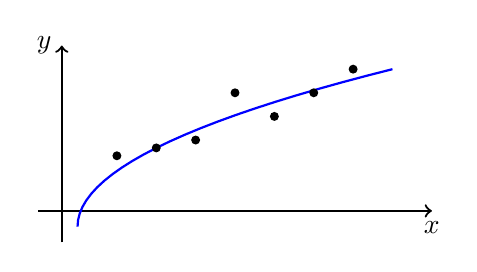
\begin{tikzpicture}[domain=0:2]
      \draw[thick,->] (-0.5,0.2) -- (4.5,0.2) node [below] {$x$};
      \draw[thick,->] (-0.2,-0.2) -- (-0.2,2.3) node [left] {$y$};
      \draw[thick,blue] plot (\x*\x,\x);
      \filldraw (0.5,0.9) circle (1.4pt);
      \filldraw (1,1) circle (1.4pt);
      \filldraw (1.5,1.1) circle (1.4pt);
      \filldraw (2,1.7) circle (1.4pt);
      \filldraw (2.5,1.4) circle (1.4pt);
      \filldraw (3,1.7) circle (1.4pt);
      \filldraw (3.5,2) circle (1.4pt);
   \end{tikzpicture}
\end{minipage}
\begin{minipage}{0.55\textwidth}
   \vspace{0.2cm}Potremmo ad esempio avere dei dati distribuiti come in figura e volerli interpolare, sapendo che la forma funzionale dovrebbe essere, ad esempio, una parabola: in questo caso essa dipenderà in generale da tre parametri.
\end{minipage}

\vspace{0.4cm}Vogliamo dunque trovare la funzione più adeguata di quel tipo di forma funzionale, la quale passa attraverso i dati nonostante non intersechi alcun punto in particolare. \E chiaro che può capitare che passi per qualcuno dei dati, ma come si evince anche dalla figura gli altri dati sono distribuiti attorno alla curva.

Da un punto di vista euristico, questa è una buona approssimazione su tutto l'insieme dei dati. In questo caso si parla di regressione, e il motivo per cui la curva è detta la più adatta è perché identifichiamo una funzione obiettivo (una funzione che vogliamo minimizzare o massimizzare, in generale ottimizzare) e andiamo a cercare i valori più adatti dei parametri $\underline{a}$ tali che la funzione è minima o massima rispetto al tipo di curva assegnata. La funzione obiettivo di cui parliamo è il $\chi^2$, la quale è definita come la differenza tra il valore misurato $y_i$ e il valore atteso $f(\underline{x}_i,\underline{a})$ elevata al quadrato:

$$\chi^2(\underline{a})
=\frac{1}{n-1} \sum_{i=0}^{n} \big[ y_i - f(\underline{x}_i,\underline{a}) \big]^2\geq0$$

Sebbene considerando il quadrato della differenza perdiamo l'informazione sul segno della differenza $y_i - f(\underline{x}_i,\underline{a})$, ciò ci permette di sapere a priori che il $\chi^2$ è una funzione non negativa, per cui è limitata dal basso: il suo minimo è 0. Inoltre, poiché tale funzione è regolare

\textbf{mi fa male la testa, continua lezione 1 14:50 circa}

$$y=f(x)=f(x_0) + f'(x_0)(x-x_0) + \frac{1}{2!}f''(x_0)(x-x_0)^2 + \ldots$$

$$\begin{cases}
   c_0 + c_1x_0 + c_2 x_0^2 + \ldots + c_n x_0^n=y_0\\
   c_0 + c_1x_1 + c_2 x_1^2 + \ldots + c_n x_1^n=y_1\\
   \vdots\\
   c_0 + c_1x_n + c_2 x_n^2 + \ldots + c_n x_n^n=y_n
\end{cases}$$

Possiamo esprimere il sistema come

$$V \underline{c}=\underline{y}$$

dove

$$V=
\begin{pmatrix}
   1 & x_0 & x_0^2 & \ldots & x_0^n\\
   1 & x_1 & x_1^2 & \ldots & x_1^n\\
   \vdots & \vdots & \vdots & \ddots & \vdots\\
   1 & x_n & x_n^2 & \ldots & x_n^n\\
\end{pmatrix}
\quad,\quad
\underline{c}=
\begin{pmatrix}
   c_0\\
   \vdots\\
   c_n
\end{pmatrix}
\quad,\quad
\underline{y}=
\begin{pmatrix}
   y_0\\
   \vdots\\
   y_n
\end{pmatrix}$$

$V$ è detta \textbf{matrice di Vandermonde}. Poiché $x_i \neq x_j \quad \forall \, i \neq j$, ogni colonna è diversa e quindi il determinante è non nullo. Per calcolarlo sottraiamo ad ogni colonna la precedente moltiplicata per $x_0$:

$$\det (V)=
\begin{pmatrix}
   1 & x_0 - x_0 & x_0^2 - x_0^2 & \ldots & x_0^n - x_0^n\\
   1 & x_1 - x_0 & x_1^2 - x_0x_1 & \ldots & x_1^n - x_0x_1^{n-1}\\
   \vdots & \vdots & \vdots & \ddots & \vdots\\
   1 & x_n - x_0 & x_n^2 - x_0x_n & \ldots & x_n^n - x_0 x_n^{n-1}\\
\end{pmatrix}$$

$$\implies \det (V)=
\begin{pmatrix}
   1 & 0 & 0 & \ldots & 0\\
   1 & x_1 - x_0 & (x_1 - x_0)x_1 & \ldots & (x_1 - x_0)x_1^{n-1}\\
   \vdots & \vdots & \vdots & \ddots & \vdots\\
   1 & x_n - x_0 & (x_n - x_0)x_n & \ldots & (x_n - x_0)x_n^{n-1}\\
\end{pmatrix}$$

dividendo la $j$-esima riga (tranne la prima) per $x_j - x_0$ e portando fuori dalla matrice otteniamo

$$\det (V)=
\begin{pmatrix}
   1 & 0 & 0 & \ldots & 0\\
   1 & 1 & x_1 & \ldots & x_1^{n-1}\\
   \vdots & \vdots & \vdots & \ddots & \vdots\\
   1 & 1 & x_n & \ldots & x_n^{n-1}\\
\end{pmatrix}
\underbrace{(x_1 - x_0) \cdot \ldots \cdot (x_n - x_0)}_{\displaystyle = \prod_{j=2}^{n} (x_j - x_0)}$$

La matrice risultante non dipende più da $x_0$. Reiterando il processo possiamo eliminare la dipendenza da ogni $x_i$ e in forma compatta il determinante si potrà scrivere come

$$\det V=\prod_{i>j} (x_i - x_j)$$

Tale espressione ci dice che se i punti sono tutti distinti il determinante della matrice è diverso da zero. Si può anche scrivere come

$$\det V=\prod_{j=0}^{n-1} \qty( \prod_{i=j+1}^{n} (x_i - x_j) )$$

\textbf{non ho capito come si passa a questo vabbè}

$$P_n(x)=\sum_{i=0}^{n} f(x_i) L_i(x)$$

dove

$$L_i(x)=\prod_{\begin{subarray}{c}
   k=0\\[0.1cm]
   k \neq i
\end{subarray}
}^{n} \frac{x - x_k}{x_i - x_k}
$$

nota: essendo così definito, il denominatore è sempre diverso da zero.

L'ordine di ogni polinomio $L_i$ è proprio $n$

$$L_i=\frac{
(x - x_0) (x - x_1) \ldots (x - x_{i-1}) (x - x_{i+1}) \ldots (x - x_n)
}{
(x_i - x_0) (x_i - x_1) \ldots (x_i - x_{i-1}) (x_i - x_{i+1}) \ldots (x_i - x_n)
}$$

Si ha che

$$L_i(x_j)=
\left\{
   \begin{array}{ll}
      0 & \text{se } j \neq i\\
      1 & \text{se } j = i
   \end{array}
\right.
\equiv \delta_{ij}$$

infatti nel primo caso a numeratore ci sarà un termine nullo, nel secondo caso numeratore e denominatore saranno uguali.

In definitiva abbiamo che

$$P_n(x_j)=\sum_{i=0}^{n} f(x_i) L_i(x_j)
=\sum_{i=0}^{n} f(x_i) \delta_{ij}
=f(x_j) \quad \forall \, j$$

\subsection{Formula di Newton per il polinomio interpolante}

Tale metodo si adopera quando abbiamo trovato la soluzione per $n$ punti e ne includiamo un altro. Supposto quindi di avere il polinomio $P_{n-1}(x)$ che passa per $x_0,x_1,\ldots,x_{n-1}$, poniamo

$$P_n(x)=P_{n-1}(x) + a_n w_{n-1}(x)$$

dove

$$w_{n-1}(x)=\prod_{i=0}^{n-1} (x - x_i)
\quad,\quad
a_n=\frac{f(x_n) - P_{n-1}(x_n)}{w_{n-1}(x_n)}$$

$w_{n-1}$ è un \textit{polinomio monico}, cioè un polinomio tale che il coefficiente del termine di grado massimo è pari a 1. Inoltre ha grado $n$.

\vspace{0.2cm}Proviamo innanzitutto che il nuovo polinomio passa per i primi $n-1$ punti.

Posto $k \leq n-1$ si ha

$$w_{n-1}(x_k)=0$$
$$P_n(x_k)=P_{n-1}(x_k) + a_n \underbrace{w_{n-1}(x_k)}_{=0}
=P_{n-1}(x_k)
\equiv f(x_k)$$

Proviamo adesso che passa per il nuovo punto:

$$P_n(x_n)=P_{n-1}(x_n) + a_n w_{n-1}(x_n)
=P_{n-1}(x_n) + \frac{f(x_n) - P_{n-1}(x_n)}{w_{n-1}(x_n)} w_{n-1}(x_n)=$$
$$=P_{n-1}(x_n) + f(x_n) - P_{n-1}(x_n)
=f(x_n) $$

$$P_n(x)=c_0 + c_1x + c_2x^2 + \ldots + c_nx^n=$$
$$=c_0 + a_1(x-x_0) + a_2(x-x_0)(x-x_1) + \ldots + a_n(x-x_0)(x-x_1)\ldots(x-x_n)=$$
$$=\sum_{k=0}^{n} a_k w_{k-1}(x)$$

\section{Errore nell'estrapolazione}

$$w_n(x)=F(x)=\prod_{k=0}^{n} (x - x_k)
\quad,\quad
F_i(x)=\prod_{
   \begin{subarray}{c}
      k=0\\[0.1cm]
      k \neq 1
   \end{subarray}
}^{n} (x - x_k)$$

Sia $\overline{x} \neq x_k$ (tra i nodi) tale che $\displaystyle a \leq \min_{k} x_k < \overline{x} < \max_{k} x_k \leq b$.

Sia

$$G(x)=f(x) - P_n(x) - RF(x)$$

dove $R$ è un parametro scelto in maniera tale che $G(\overline{x})=0$. $G$ è uguale all'errore ma corretto con $F(x)$. Si ha che

$$G(x_k)=f(x_k) - P_n(x_k) - RF(x_k)=0
\quad \forall \, x_k \;,\; k=0,1,\ldots,n$$

perché è una nodal function. Ne segue che $G(x)$ si annulla in $n+2$ punti: $x_0,x_1,\ldots,\overline{x},\ldots,x_n$. Per il teorema di Rolle, $G'(x)$ si annullerà in $n+1$ punti intermedi. Reiterando tale teorema otteniamo che $G^{(n+1)}(x)$ si annullerà in un solo punto $\xi \in [a,b]$. D'altra parte:

\begin{itemize}
   \item $P_n(x)$ è un polinomio di grado minore o uguale $n$, per cui $P^{(n+1)}=0$;
   \item $F(x)$ è un polinomio monico di grado $n+1$, dunque $F^{(n+1)}(x)=(n+1)!$
\end{itemize}

In definitiva:

$$G^{(n+1)}(x)=f^{(n+1)}(x) + 0 - R(n+1)!$$

Abbiamo visto che

$$\exists \, \xi : G^{(n+1)}(\xi)=f^{(n+1)}(\xi) - R(n+1)!=0
\implies
R=\frac{f^{(n+1)}(\xi)}{R(n+1)!}$$

$$\implies G(x)=f(x) - P_n(x) - \eval{\frac{f^{(n+1)}(\xi)}{(n+1)!} F(x)}_{x=\overline{x}}=0$$

$$f(x)=P_n(x) + \frac{f^{(n+1)}(\xi)}{(n+1)!} w_n(x)$$

\subsection{Prodotto scalare (prodotto hermitiano)}

Applicazione lineare $\braket*{\, \cdot \, }{\, \cdot \,}:V \times V \to \mathbb{C}$

\begin{enumerate}[label=(\roman*)]
   \item $\braket*{u}{v}=\braket*{v}{u}^*$
   \item $\braket*{u}{\lambda_1 v_1 + \lambda_2 v_2}=\lambda_21\braket*{u}{v_1} + \lambda_2 \braket*{u}{v_2}$
   
   $\braket*{\lambda_1 u_1 + \lambda_2 u_2}{v}=\lambda^*_2 \braket*{u_1}{v} + \lambda^*_2 \braket*{u_2}{v}$
   \item $\braket*{u}{u} \geq 0$, $\braket*{u}{u}=0 \iff u=0$
\end{enumerate}

\subsection{Polinomi di Legendre}

$$\braket*{\phi_k}{\phi_{k'}}c_{k'}
=\braket*{\phi_k}{v}$$

$$\begin{pmatrix}
   \braket*{\phi_0}{\phi_0} & \braket*{\phi_0}{\phi_1} & \ldots & \braket*{\phi_0}{\phi_n}\\
   \vdots &\vdots & \ddots & \vdots\\
   \braket*{\phi_n}{\phi_0} & \ldots & \ldots & \braket*{\phi_n}{\phi_n}
\end{pmatrix}
\begin{pmatrix}
   c_0\\
   \vdots\\
   c_n
\end{pmatrix}
=
\begin{pmatrix}
   \braket*{\phi_0}{v}\\
   \vdots\\
   \braket*{\phi_n}{v}
\end{pmatrix}$$

$$\| \phi_0 \|^2
=\braket*{\phi_0}{\phi_0}
=\int_{-1}^{1} 1 \cdot 1 \dd{x}=2
\implies
\tilde{P}(x)=\frac{1}{\sqrt{2}}$$

Dunque il primo polinomio di Legendre è ancora una costante.

$$\tilde{P}_1=\phi_1 - \hat{P}_0 \braket*{\hat{P}_0}{\phi_1}=\phi_1=x$$

$$\braket*{\hat{P}_0}{\phi_1}=\int_{-1}^{1} \frac{1}{\sqrt{2}} x \dd{x}=0$$

(perché l'integranda è dispari e l'intervallo è simmetrico)

$$\implies \hat{P}_1
=\frac{x}{\displaystyle \sqrt{\frac{2}{3}}}
=\sqrt{\frac{3}{2}}x$$

$$
\begin{array}{lcccc}
   k && p_k(x) \text{ (ortogonali)} && \hat{p}_k(x) \text{ (ortonormali)}\\[0.2cm]
   0 && 1 && \displaystyle \sqrt{\frac{1}{2}}\\[0.4cm]
   1 && x && \displaystyle x \sqrt{\frac{3}{2}}\\[0.4cm]
   2 && \displaystyle \frac{3x^2 - 1}{2} && \displaystyle \frac{3x^2 - 1}{2} \sqrt{\frac{5}{2}}\\[0.4cm]
   3 && \displaystyle \frac{5x^3 - 3x^2}{2} && \displaystyle \frac{5x^3 - 3x^2}{2} \sqrt{\frac{7}{2}}\\[0.4cm]
   4 && \displaystyle \frac{35x^4 - 30 x^2 + 2}{8} && \displaystyle \frac{35x^4 - 30 x^2 + 2}{8} \sqrt{\frac{9}{2}}\\[0.4cm]
\end{array}$$

\subsubsection{Sviluppo in multipolo}

$$V(\underline{r})=\frac{1}{4 \pi \varepsilon_0} \int_{\Omega} \frac{\rho(\underline{r}')}{| \underline{r} - \underline{r}' |} \dd[3]{\underline{r}'}$$

$$Q=\int_{\Omega} \rho(\underline{r}') \dd[3]\underline{r}'$$

Il potenziale allora sarà

$$V(\underline{r}) \approxeq \frac{1}{4 \pi \varepsilon_0}\frac{Q}{r}$$

$$\frac{1}{| \underline{r} - \underline{r}' |}
=\frac{1}{\sqrt{r^2 + r'^2 - 2 r r' \cos{\vartheta}}}$$

$$r_{>}=\max \qty{r,r'}
\quad,\quad
r_{<}=\min \qty{r,r'}$$

Supponiamo che $\underline{r} \neq \underline{r}' \iff \underline{r} - \underline{r}' \neq 0$

$$\frac{1}{| \underline{r} - \underline{r}' |}
=\frac{1}{r_{>} \displaystyle \sqrt{1 - 2\frac{r_{<}}{r_{>}} \cos{\vartheta} + \qty(\frac{r_{<}}{r_{>}})^2}}$$

Consideriamo l'espansione di Taylor

$$\frac{1}{\sqrt{1 + x}}=1 - \frac{1}{2}x + \frac{1 \cdot 3}{2 \cdot 4} x^2 - \frac{1 \cdot 3 \cdot 5}{2 \cdot 4 \cdot 6} x^3
\quad \text{per } |x|<1$$

Se poniamo

$$x=- 2\frac{r_{<}}{r_{>}} \cos{\vartheta} + \qty(\frac{r_{<}}{r_{>}})^2$$

\subsection{Funzione generatrice per polinomi ortonormali}

Siano $\qty{P_n}$ un insieme di polinomi ortogonali e normalizzati rispetto ad un peso dato \textbf{sta parte mi sembra poco chiara}

Si avrà

$$\delta_{nm}=\braket*{P_n}{P_m}
=\int_{a}^{b} P_n(x) P_m(x) w(x) \dd{x}$$

$$\braket*{Q_{n-1}}{P_n}
=\int_{a}^{b} P_n(x) Q_{n-1}(x) w(x) \dd{x}=0$$

$$U_n(x): \quad w(x) P_n(x)=\dv[n]{U_n(x)}{x}$$

$$\int_{a}^{b} Q_{n-1}(x) w(x) P_n(x) \dd{x}=0$$

$$0=\int_{a}^{b} Q_{n-1}(x) \dv[n]{U_n(x)}{x} \dd{x}$$

Tale integrale può essere risolto integrando per parti $n$ volte. La prima volta si ha

$$=\qty[Q_{n-1}(x) \dv[n-1]{U_n(x)}{x}]_{a}^{b}
- \int_{a}^{b} Q'_{n-1}(x) \dv[n-1]{U_n(x)}{x} \dd{x}$$

($Q'_{n-1}(x)$ ha grado $n-2$). Reiterando il processo si ha

$$=\Big[ Q_{n-1}(x) U_n^{(n-1)}(x) - Q'_{n-1}(x) U_n^{(n-2)}(x) + $$
$$+Q''_{n-1}(x) U_n^{(n-3)}(x) + \ldots + (-1)^{n-1} Q^{(n-1)}_{n-1}(x) U_n(x) \Big]_{a}^{b}$$

$$\begin{cases}
   U_n(a)=U_n'(a)=\ldots=U_n^{(n-1)}(a)=0\\[0.1cm]
   U_n(b)=U_n'(b)=\ldots=U_n^{(n-1)}(b)=0\\
\end{cases}$$

$$P_n(x)=\frac{1}{w(x)} \dv[n]{U_n(x)}{x}$$

(Si può fare perché $w>0 \quad \forall \, x \in [a,b]$)

Tale espressione è un polinomio di grado $n$, che se viene differenziato $n+1$ volte diventa 0:

$$P_n^{(n+1)}=0$$

Segue che

$$\dv[n+1]{x} \qty[ \frac{1}{w(x)} \dv[n]{U_n(x)}{x} ]=0$$

$$\dv[2n+1]{x} U_n(x)=0$$

$$\begin{cases}
   U_n(-1)=U_n'(-1)=\ldots=U_n^{(n-1)}(-1)=0\\[0.1cm]
   U_n(1)=U_n'(1)=\ldots=U_n^{(n-1)}(1)=0\\
\end{cases}$$

$$U_n(x)=c_n (x^2 - 1)^n$$

$$P_n(x)=c_n \dv[n]{x} (x^2 - 1)^n
=c_n \dv[n]{x} \big[ (x + 1)^n (x - 1)^n \big]=$$
$$=c_n \qty[ (x+1)^n \dv[n]{x} (x - 1)^n + n \dv{x} (x+1)^n \dv[n-1]{x} (x-1)^n + \ldots]$$

Si ha che

$$\dv[n]{x} \eval{(x-1)^n}_{x=1}
=\dv[n]{x} \eval{(x^n + \ldots )}_{x=1}=n!$$

(solo il primo termine termine sopravvive, diventando una costante pari a $n!$)

per gli altri termini invece si ha

$$\dv[n-k]{x} \eval{(x-1)^n}_{x=1}=0 \quad \forall \, k>2$$

Dunque

$$P_n(1)=c_n 2^n n! + 0$$

Se imponiamo la condizione $P_n(1)=1$ si ottiene

$$c_n 2^n n!=1
\implies
c_n=\frac{1}{ 2^n n! }$$

Allora il generico polinomio di Legendre sarà definito come

$$P_n(x)=\frac{2}{ 2^n n! } \dv[n]{x} (x^2 - 1)^n$$

\subsection{Formule ricorsive}

Esse sono formule che permettono di trovare un polinomio in un certo punto $x$ avendo alcuni polinomi calcolati nello stesso punto ma con indice minore (ad esempio per trovare $P_n$ ci serve $P_{n-1}$ e $P_{n-2}$). Quindi piuttosto che derivare diverse volte la funzione generatrice si può partire da alcuni polinomi e combinarli per ottenere i successivi.

Per ottenere la formula si parte dall'identità

$$\phi(t,x)=\frac{1}{\sqrt{1 - 2xt + t^2}}$$

Essa è simile a

$$\frac{1}{| \underline{r} - \underline{r}' |}
=\frac{1}{r_{>} \displaystyle \sqrt{1 - 2\frac{r_{<}}{r_{>}} \cos{\vartheta} + \qty(\frac{r_{<}}{r_{>}})^2}}
\quad\text{con}\quad
\begin{cases}
   \displaystyle t=\frac{r_{<}}{r_{>}}\\[0.4cm]
   \cos{\vartheta}=x
\end{cases}$$

di cui abbiamo ricavato l'espansione in multipolo. Essa sarà:

$$\phi(t,x)=\sum_{l=0}^{\infty} P_l(x) t^l$$

$$\pdv{\phi}{t}
=-\frac{1}{2} \frac{-2x+2t}{(1-2xt+t^2)^{\frac{3}{2}}}
=\phi(t,x) \frac{x - t}{1-2xt+t^2}
=\frac{x - t}{1-2xt+t^2} \sum_{l=0}^{\infty} P_l(x) t^l$$

$$\pdv{t} \sum_{l=0}^{\infty} P_l(x) t^l
=\sum_{l=0}^{\infty} P_l(x) l t^{l - 1}$$

Le derivate dei due termini devono essere uguali, quindi:

$$\sum_{l=0}^{\infty} l P_l(x) t^{l - 1}
=\frac{x-t}{1 - 2xt + t^2} \sum_{l=0}^{\infty} P_l(x) t^l$$

Per poter scrivere tutto come un unico polinomio in $t$ e porre i coefficienti di tale polinomio uguali a zero (principio di identità dei polinomi) moltiplichiamo entrambi i termini per $(1 - 2xt + t^2)$:

$$(1 - 2xt + t^2)\sum_{l=0}^{\infty} l P_l(x) t^{l - 1}
=(x - t) \sum_{l=0}^{\infty} P_l(x) t^l$$

Nella sommatoria del primo membro, il termine per $l=0$ è nullo, quindi possiamo partire da $l=1$. Per partire comunque da $l=0$ scriviamo

$$(1 - 2xt + t^2)\sum_{l=0}^{\infty} (l + 1) P_{l + 1}(x) t^{l +1 - 1}
=(x - t) \sum_{l=0}^{\infty} P_l(x) t^l$$

cioè a sinistra partiamo da $l+1$ anziché da $l$. Avendo due sommatorie simili possiamo raggrupparle e, moltiplicando per i rispettivi fattori davanti alle sommatorie, si ha

$$\sum_{l=0}^{\infty} \big[ (l + 1)P_{l + 1}(x) t^l - 2(l + 1)x P_{l + 1}(x) t^{l+1} +$$
$$+ (l + 1)P_{l+1}(x)t^{l+2} - x P_l(x)t^l + P_l(x)t^{l+1} \big]=0
\quad \forall \, x,t$$

Raggruppiamo i termini con la potenza di $t$:

$$\sum_{l=0}^{\infty} \Big\{ \big[ (l+1)P_{l+1}(x) - xP_l(x) \big] t^l + \big[ P_l(x) -2(l+1)xP_{l+1}(x) \big]t^{l+1} + (l+1)P_{l+1}(x)t^{l+2} \Big\}=0$$

\subsection{Approssimazione di integrali}

$$f(x)=y_k + \frac{y_{k+1} - y_k}{x_{k+1} - x_k} (x - x_k)
=y_k + \underbrace{\frac{y_{k+1} - y_k}{h}}_{\approx f'_k + o(h)} (x - x_k)$$

$$\int_{x_k}^{x_{k+1}} f(x) \dd{x}
=\int_{x_k}^{x_{k+1}} \qty{ y_k + \Big( \frac{y_{k+1} - y_k}{h} + o(h) \Big)(x - x_k) } \dd{x}=$$
$$=y_k(x_{k+1} - x_k) + \qty[ \frac{y_{k+1} - y_k}{h} + o(h) ]\qty[ \frac{(x - x_k)^2}{2} ]_{x_k}^{x_{k+1}}$$

\subsection{Il modello di Ising}

Il modello di Ising è un modello per il magnetismo nato per spiegare la transizione da una fase magnetica all'altra passando da un regime a temperatura più bassa ad uno a temperatura più alta in cui molti spin, molti momenti magnetici si orientano nella stessa direzione. Sia $i$ un nodo e $S_i$ il relativo spin. Ising fece un modello monodimensionale in cui abbiamo una sola linea con i nodi isolati, e ogni relativo spin si assume possa essere diretto solo verso l'alto o verso il basso ($+1$ e $-1$)

\begin{center}
   \begin{tikzpicture}[scale=1.5]
      \draw (-2,0) -- (2,0);
      \draw[thick,->] (-0.5,-0.2) -- (-0.5,0.2);
      \draw[thick,->] (0.5,0.2) -- (0.5,-0.2);
      \node at (4,0) {$S_i \in \qty{+1,-1}$};
   \end{tikzpicture}
\end{center}

Gli spin interagiscono tra loro, ma per semplicità assumiamo che possono interagire solo due spin tra loro vicini.

L'energia del sistema può crescere o decrescere a seconda che il loro prodotto sia positivo o negativo.

L'hamiltoniana del sistema per l'energia si scrive come

$$\mathcal{H}=\sum_{\expval{ij}} J_{ij} S_i S_j
\quad\text{dove}\quad
J_{ij}=\left\{
   \begin{array}{lc}
      +J & \rm AFM\\
      -J & \rm FM
   \end{array}
\right.$$

La scrittura $\expval*{ij}$ indica che consideriamo soltanto l'interazione tra spazi vicini. I due valori di $J_{ij}$ rappresentano un sistema ferromagnetico (FM) e uno anti-ferromagnetico (AFM), cioè quando gli spin sono paralleli (entrambi +1 o entrambi -1)

$$\mathcal{H}=\sum_{\expval{ij}} J_{ij} S_i S_j - H \sum_{i} S_i$$

$$m=\frac{1}{N} \sum_{i} S_i$$

$$\expval*{o}=\frac{1}{z} \sum_{S} o(S) e^{-\frac{H(S)}{k_b T}}$$

\section{Best fit}
Consider 
\[(\underline{x_i},\underline{y_i}), x_p \in R^p, y \in R, \forall i=1,...,n \] 
\[ y=f(\underline{x},\underline{a}) \; \; \underline{a} \in R^p\]
y is a funcional form.
The problem is finding the most likely value that interpolate given values, doing this is called best fit.
So now Consider:\[x^2(\underline{a}=\frac{1}{n}\cdot \sum [y_i-f(\underline{x_i},a)]^2)\] we have to find the minimum. 

\subsection{Taylor expantion}
If we know well the function until a certain point we can consider
\[f(0),f'(o),f"(0)\] 
Taylor expantion allow us to write:
\[f(x)=f(0)+f'(0)+\frac{1}{2!}f"(0)+R(x)\]
Where R is the discrepancy, so we have an error that can be extimated using R.

\section{Weierstrass approximation theorem}
Is an existence theorem. Let's consider 
\[f:[a,b] \rightarrow R \; \; c^0:([a,b])\]
Therefore exist a set of polynomial funcion $P^{(x)}_n$ con $n=0,1,...$ and this polynomials approcximate the given function
Possiamo quindi con un errore piccolo approssimare asintoticamente la funzione a un polinomio. Osserviamo:
\[\lim_{n\to +\infty}(max |{f(x)-P^{x}_n}|)=0\]

So we have a sequence of non negative number and this sequences goes to 0 as n goes to infinity.
 
\subsection{Interpolating polynomials}
In the point we know the exacto value of the function but in between we don't mind.
let's consider 
\[n+1 \; x_i \; i=0,...,n\]
\[f(x_i)=y_i\]
find the Interpolating polynomial:
\[P_n(x) \in R^n[x]=\{P_k(x) \; : \; k=degP_k(x)\le n\}\]
L'insieme è un set di funzioni polinomiali.
\\
$dimR^N[x]=n+1 \rightarrow [1,x,x^2,...,x^n]$  is a linear space. Allora possiamo scrivere il polinomio:
\[P_k(x)=c_0+c_1(x)+c_2(x^2)+...+c_k(x^k) \; \; |; 0\le k \le n\] tale che $P_n(x_i)=f(x_i)$ is the exacti value of the function at the point (we only care at the point).
Under the condition that $x_i \neq x_j \;\; i \neq j$ the polynomial exist and is unic (this is an assumpion).
\\
Scriviamo adesso:\[P_n(x)=c_0+c_1(x)+c_2(x^2)+...+c_n(x^n)\] someone of this coefficient can be zero. So let's suppose that $\sum|c_i|>0$ (cioè che non tutti sono zero)
$$\begin{cases}
 C_0+c_1(x_0)+c_2(x^2_0)+\cdot+c_n(x^n_0)=y_0 \\
C_0+c_1(x_1)+c_2(x^2_1)+.\cdot+c_n(x^n_1)=y_1 \\
C_0+c_1(x_n)+c_2(x^2_n)+\cdot+c_n(x^n_n)=y_n \\ 
\end{cases}$$
\\
It's a linear sistem of n+1 equation, in general is a non omogenean sistem. For costruction:
\[P_n(x)-f(x)|_{x=x_i}=0\]
\section{Vandermond Matrix}
$V(x_0,...x_n)$
$$
\begin{array}{|c c c c c|}
   1  &x_0 & x^2_0 &...&x^n_0 \\ 
1  & x_1 & x^2_1 &...&x^n_1 \\
...  &... & ... &...&...\\
1  &x_n & x^2_n &...&x^n_n  
\end{array}$$
This matrix is well known in Algebra, it's called Vandermonde matrix.
Under the condition that \[x_i\neq x_j \;\; i \neq j \; \rightarrow detV(\underline{x}) \neq 0\]
if we consider a polynomial like:
$$P_n(x)=\sum f(x_i) L_i(x)$$
where:
$$L_i(x)= \prod^n_{k=0}\frac{x-x_n}{x_i-x_k}$$ di grado n.

$$L_i(x_j)= \begin{cases}
    0 & j \neq i\\
    1 & j=i
\end{cases} = \delta_{ij}$$

infatti:
$$P_n(x)=\sum^n f(x_i)L_i(x_j)=\sum f(x_i) \delta_{ij}=f(x_j)$$
Allora possiamo modificare il determinante di Vandermonde in una matrice che abbia lo stesso valore:
$$DetV=\begin{array}{|cc|}
     &  \\
     & 
\end{array}$$
e possiamo fattorizzare:
$$=(x_1-x_0)(x_2-x_o)\ldots(x_n-x_0) \ldots \begin{array}{|cccc|}
   1  &x_1  & \ldots &x^{n-1}_1\\
    1  &x_2  &\ldots&x^{n-1}_2\\
    \ldots  & \ldots &\ldots &\ldots\\
      1  &x_n  &\ldots&x^{n-1}_n\\
\end{array}$$
Ripetendo questo processo alla fine troveremo che:
$$DetV=\prod_{i>j}(x_i-x_j)$$

\section{Lagrange Form}
Sia: $$P_n(x)=\sum^n f(x_i)L_i(x) \in R^n[x]$$
Dove $R^n$ è uno spazio lineare di grado non maggiore di n, $f(x_i)$ sono i valori della funzione data , e $L_i(x)$ is the given polynomial.
\section{Newton form}
Newton form is another form for polynomian of given order. Serve nel caso in cui dati n dati voglia aggiungerne altri, una volta aumentato il numero di dati cambierà anche il polinomio di base.

Let's consider $P_{n-1}(x) passing through \; \; x_0,x_1,..,x_{n-1}$ e $P_n(x) \; \; x_0,x_1,..,x_n$ we want to know if exist a formula that mette in relazione questi due polinomi. Usiamo the divided diffrences method (Newton):
$$P_n(x)= P_{n-1}(x)+a_n w_{n-1(x)}$$ where $$w_{n-1}=\prod^{n-1}_{i=0}(x-x_i)= 1\cdot x^n+...$$ cioè a monic polynomial che sono polinomi il cui termine di massimo grado ha coefficiente uno. IL gradi di questa funzione è n (da zero a n+1).
\\
Definiamo adesso:
$$a_n=\frac{f(x_n)-P_{n-1}(x_n)}{w_{n-1}(x_n)}$$
consideriamo $k \le n-1$ e proviamo che il nuovo polinomio passa per i punti.
\[w_{n-1}(w_k)=0\] uno dei termini della produttotia sarà $x_k-x_k$
\[P_n(w_k)=P_{n-1}(w_k)+a_nw_{n-1}(w_k)=P_{n-1}(w_k)=f(x_k)\]
The only condition to fullfill is that passes through the new point
\[P(x_n)=P_{n-1}(x_n)+a_nw_{n-1}(x_n)=P_{n-1}(x_n)+\frac{f(x_n)-P_{n-1}(x_n)}{w_{n-1}(x_n)}w_{n-1}(x_n)=f(x_n)\]
\[P_n(x)=c_0+c_1+c_2x^2+...+c_nx^n=c_0+a_1(x-x_0)+a_2(x-x_0)(x-x_1)+...+a_n(x-x_0)(x-x_1)...(x-x_n)\]
\[=\sum a_kx_{k-1}(x)\]
    
\section{Shamir's secret Shary}
Immaginiamo di avere un informazione e $S_1,...,S_n$ executive officers, per conoscere l'informazione solo k di essi saranno necessari con $s \le n$.
Sia $a_0=S$ la nostra informazione, costruiamo il polinomio:
\[f(x)=a_0+a_1x+ \cdots + a_{k-1}x^{k-1}\]
questo polinomio sarà univocamente determinato se conosco il valore in k punti, allora posso trovare $a_0$ e conseguentemente S.q
uesto polinomio prodece:
\[S_i=(i,f(i)) \; \; with \; \; 1 \le i \le n\] cioè la iesima informazione che verrà assegnata all'executive officer.

\section{Point error in Lagrange interpolation}
Siano:
\[f:[a,b]\rightarrow R \;\;\; f \in C^{n-i}([a,b])\]
\[x_0,...,x_n \in [a,b] \;\;\; y_l=f(x_k)\]
\[P_n(x)= \sum^n y_iL_i(x) \;\;\;\; where ;\; L_i=\prod^N \frac{x-x_k}{x_i-x_k}\]
\[F(x)=\prod^n(x-x_k) \;\;\; F_i(x)=\prod(x-x_k)=(x-x_i)F_i(x)\]
\[F'(x)=(x-x_i)F'_i(x)+F_i(x)\]
\[F'(x_i)=F_i(x_i)\neq 0\]
\[L_i(x)=\prod^n \frac{x-x_k}{x_i-x_k}=\frac{\prod x-x_k}{\prod x_i-x_k}=\frac{F_i(x)}{F_i(x_i)}=\frac{F(x)}{(x-x_i)F'(x)}\]
so we can write:
\[P_n(x)=\sum^n y_i \frac{F(x)}{(x-x_k)F'(x_k)}\] con \[\overline x\neq x_k \;\;\; a \le minx_k < \overline{x} < maxx_k \le b\]
\[G(x)=f(x)-P_n(x)-RF(x) \;\;\; R:G(x)=0\]   
\[G(x_k)=f(x)-P_n(x_k)-RF(x_i)=0\] i primi due termini del secondo membro si annullano in quanto sono uguali perchè Pn interpola f, il terzo termine è zero per costruzione di F.
Troviamo quindi che G(x) vanish at n+2 points, allora per il teorema di rolle la derivata di g si annulla in n+1 punti. 
\\
\[G^{n+1}(\xi)=f^{n+1}(x)-R(n+1)!\]
\[\exists \xi \in [a,b] : G^{n+1}(\xi)=0 \; \rightarrow G^{n+1}(\xi)=f^{n+1}(x)-R(n+1)!=0 \] Allora R può essere espresso come: 
\[R=\frac{f^{n+1}(\xi)}{(n+1)!}\]
Allora:
\[G(x)=f(x)-P_n(x)-\frac{f^{n+1}(\xi)}{(n+1)!}F(x)|_{x=\overline x}=0\]
e per la stima dell'errore in un punto:
\[f(x)=P_n(x)+\frac{f^{n+1}(\xi)}{(n+1)!}F(x)\]
\\
Cosa succede se i punti collassano in uno solo?
siano:
\[x_0=x_0 \;\; x_1=x_0+h \;\; x_1=x_0+2h \;\; x_n=x_0+nh\] given point, con
\[x_1-x_0=h \;\;x_2-x_0=2h \;\;x_n-x_0=nh \]

\[x=x_0+Sh \;\;\; S<h\]
allora:
\[w_n(x)=(x-x_0)(x-x_1)...(x-x_n)=(x_0+Sh-x_0)(x_0+Sh-x_0-h)...(x_0+Sh-x_0-nh)=h^{n+1}S(s-1)...(S-n)\]
sia:
\[f\in C^{n+1}([a,b])\rightarrow |f^{n+1}(\xi)|<M\]
\[|S-J|\le |S|+|J|<n+n=2n\]
\[h=\frac{b-a}{n}\]

\section{Runge Phenomenon}
\[f(x)=\frac{1}{1+25x^2}\]
goes to zero algebraically

\section{Othogonal polynomials (or orthonormal)}
sia V a linear space over a field, we can endaw:
\[:V\times V \rightarrow C\]


\section{Gram-Schmidt}
$\{\phi_k\}$ linearlmente indipendente costituisce una base dello spazio dei polinomi di non superiore a n-1
siano 
\[K=0,...,N \;\;\; k=0 \;\;\; \tilde{p_0}=\phi_0\] possiamo normalizzarlo:
\[\hat{p_0}=\frac{\tilde{p_0}}{||\tilde{p_0}||}\]
in particular \[||\tilde{p_0}||^2=\]

sia $k>0$ definiamo 
\[\tilde{p_k}=\phi_k-\sum_{k'<k}\hat{p_{k'}}brak\hat{p}\phi_k\]
\[\hat{p_1}=\frac{\tilde{p_1}}{||\tilde{p_1}||}\]
siano $f,g \in C^0([a,b])$
\[(f,g)=\int^b_a f^*(x)g(x)w(x)dx\] (f+ è il coniugato)
and w(x) is a weight function

\section{Legendre Polynomials} 
\[w(x)=1 \;\;\; [a,b]=[-1,1] \;\; \braket*{f}{g}=\int^1_{-1}f(x)g(x)dx\] 
Queste ultime sono funzioni reali chiamate Polinomi di Legendre.
iniziamo dalla base $\{\phi_k\}=\{1,x,x^2,...,x^n\}$ 
\[\tilde{p_0}=\phi_0=1\]
we have to normalize \[||\tilde{p_0}||^2=1|1=\int_{-1}^{1}1\cdot 1 dx=1\]
\[\hat{p_0}=\frac{1}{\sqrt{2}}\] è il primo polinomio di legendre, definito da una costante.
\[\tilde{p_1}=x-\frac{1}{\sqrt{2}}\int_{-1}^{1}\frac{1}{\sqrt{2}}xdx=x\]
\[||\tilde{p_1}||^2=\int_{-1}^{1}x^2dx=\frac{2}{3}\]
\[\tilde{p_1}(x)=\sqrt{\frac{3}{2}}x\]
\[\tilde{p_2}(x)=\phi_2-\hat{p_0} \braket*{\hat{p_0}}{\phi_2}-\hat{p_1}\braket*{\hat{p_1}}{\phi_2}=x^2-\frac{1}{\sqrt{2}}\int_{-1}^{1}\frac{1}{\sqrt{2}}x^2dx-\sqrt{\frac{1}{2}}x x^2 dx=x^2-\frac{1}{3}\]
\[||\tilde{p^2_2}||=\int_{-1}^{1}(x^2-\frac{1}{3})^2dx=\]
\[\tilde{p_2}(x)=\sqrt{\frac{5}{2}}(x^2-\frac{1}{3})\]
\[\tilde{p_3}(x)=\phi_3-\hat{p_0}\braket*{\hat{p_0}}{\phi_3}-\hat{p_1}\braket*{\hat{p_1}}{\phi_3}-\hat{p_2}\braket*{\hat{p_2}}{\phi_3}=x^3-\frac{3}{5}x\]
\[\tilde{p_3}(x)=\sqrt{\frac{7}{2}}(x^3-\frac{3}{5}x)\]
\[\tilde{p_4}(x)=\phi_4-\hat{p_0}\braket*{\hat{p_0}}{\phi_4}-\hat{p_1}\braket*{\hat{p_1}}{\phi_4}-\hat{p_2}\braket*{\hat{p_2}}{\phi_4}-\hat{p_3}\braket*{\hat{p_3}}{\phi_4}=x^4-\frac{6}{7}x^2+\frac{3}{35}\]
\[\tilde{p_4}(x)=\sqrt{\frac{9}{2}}(x^4-\frac{6}{7}x^2+\frac{3}{35})\]
Sono tutti polinomi reali e compresi tra -1 e 1. Fatto che non era scontato.
\\
Sia $deg\hat{p_k}=k$
\[||p_k||^2=\int_{-1}^{1}p^2_k(x)dx=\frac{2}{2k+1}\]
\[\hat{p_k}(x)=\sqrt{\frac{2k+1}{2}}p_k(x)\]

\section{Multipole expansion}
\[\frac{1}{|\underline{r}-\underline{r'}|}=\frac{1}{r}\frac{1}{\sqrt{1-2\frac{r_<}{r_>}cos\theta+\frac{r_<}{r_>}^2}}=\frac{1}{r_>}\frac{1}{\sqrt{1+x}}\]
Mc Laurin expansion:
\[\frac{1}{\sqrt{1+x}}=1-\frac{1}{2}x+\frac{3}{8}x^2-\frac{5}{16}x^3+\frac{35}{128}x^4+...\] e ottengo che:
\[\frac{1}{|\underline{r}-\underline{r'}|}=\frac{1}{r}\sum_{l=0}^{\infty}\frac{r_<^l}{r_>^{l+1}}P_l(cos\theta)\] che è la multipole expansion.
The potence generated is basicalli definded by the Legendre polynomials(?) basic approssimation.
sia $p=p(\theta)=|P_l cos\theta|$

consideriamo adesso la funzione:
\[f(x)=e^{x}=1+x+\frac{x^2}{2!}+ ...\]
questa converge sempre. Se volessimo costruire lo sviluppo con i multipoli avremmo:
\[=a_0\tilde{p_0}(x)+a_1\tilde{p_1}(x)+a_2\tilde{p_2}(x)+...\]
\[a_k=\braket*{f(x)}{\tilde{p_k}(x)}=\int_{-1}^{1}e^x\tilde{p_k}(x)dx=(e-\frac{1}{e})\sqrt{\frac{1}{2}}\]
e quindi avremo come coeficienti:
\[k:a_k\]
\[0:\sqrt{\frac{1}{2}}\]
\[1: \sqrt{\frac{3}{2}}\]
\[2: \sqrt{\frac{5}{2}}\]
\[3: \sqrt{\frac{7}{2}}\]
i coefficienti vanno a decrescere, basterà tener conto dei primi termini per avere una buona approssimazione.

\section{Generaty function}
Si considerino \[\{P_n\} \;\; w(x)\;\; [a,b] \;\; \braket*{P_n}{p_m}=\delta_{nm}\]
Any set of othonormal polynomials is a set of l.i. polynomials so is a basis of the linear space of polynomials of degree less than n.
$degQ_{n-i}=n-1$ dove :
\[Q_{n-1}=\sum_{k=0}^{\infty}q_kp^k\] una serie di potenze, allora se siamo in grado di trovare una funzione del tipo:
\[U_n(x):w(x)P_n(x)=\frac{d^nU_n(x)}{dx^n}=U_n^{(x)}(x)\]
allora abbiamo trovato la funzione generatrice.
\[0=\int_{a}^{b}Q_{n-1}(x)\frac{d^nU_n(x)}{dx^n}=\big[Q_{n-1}(x)\frac{d^{n-1}U_n(x)}{dx^{n-1}}\big]^b_a-\int_{a}^{b}Q_{n-1}(x)\frac{d^{n-1}U_n(x)}{dx^{n-1}}dx=\]
\[= \big[ Q_{n-1}(x)U^{n-1}_n(x)-Q'_{n-1}(x)U^{n-2}_n(x)+Q''_{n-1}(x)U^{n-3}_n(x)+...+(-1)^{n-1}q^{n-1}_{n-1}(x)U_n(x)\big]_a^b\]

$$\begin{cases}
   U_n(a)=U'_n(a)=...=U_n^{n-1}(a)=0 \\
   U_n(b)=U'_n(b)=...=U_n^{n-1}(b)=0 \\
\end{cases}$$
\[0=\frac{d^{n+1}}{dx^{n+1}}P_n(x)=\frac{d^{n+1}}{dx^{n+1}}(\frac{1}{w(x)}\frac{d^nU_n(x)}{dx^n})\]

$$\begin{cases}
   \frac{d^{n+1}}{dx^{n+1}}(\frac{1}{w(x)}\frac{d^nU_n(x)}{dx^n})=0 \\
   U_n(a)=U'_n(a)=...=U_n^{n-1}(a)=0 \\
   U_n(b)=U'_n(b)=...=U_n^{n-1}(b)=0 \\
\end{cases}$$
Quindi $U_n$ sarà caratteorizzata dalla prima equazione differenziale ordinaria di ordine 2n+1.

\section{Funzione generatrice dei polinomi di Legendre}
\[w(x)=1 \;\;\; a=-1 \;\;\; b=1\]
$$\begin{cases}
   U_n^{n+1}(x)=0 \\
   U_n(-1)=U'_n(-1)=...=U_n^{n-1}(-1)=0 \\
   U_n(1)=U'_n(1)=...=U_n^{n-1}(1)=0 \\
\end{cases}$$
\[P_n(x)=\frac{d^n}{dx^n}U_n(x) \rightarrow U_n(x) \in R^{2n}[x]\]
\[degU_n=2n \;\;\; U_n(x)=c_n(x^2-1^n)\]
Il membro tr parentesi si annulla dal fatto che $a=-1 \;\; b=1$
\[P_n(x)=c_n \frac{d^n}{dx^n}(x^2-1)N=c_n\frac{d^n}{dx^n} [(x+1)^n(x-1)^n]=C_n \] Bowie 

\section{Rodriguez formula}
\[P_n(x)=\frac{1}{2^n n!}\frac{d^n}{dx^n}(x^2-1)^n\]
che è la funzione generatrice dei polinomi di Legendre. 
\subsection{Qualcosa sui multipoli}
\[\frac{1}{\sqrt{1-2xt+t^2}=\sum_{l=0}^{\infty}P_l(x)t^2} \;\; |t|<1\]
where $x=cos\theta \;\; t=\frac{r_<}{r_>}$
$$F(t,x)$$

\[\pdv{F}{t}=- \frac{1}{2} \frac{-2x+2t}{1-2xt+t^2}=\frac{x-t}{1-2xt+t^2}F(t,x)=\frac{x-t}{1-2xt+t^2}\sum_{l=0}^{\infty}P_l(x)t^l\]
\[\pdv{F}{t}=\sum_{l=0}^{\infty}P_l(x)lt^{l-1}\]
\[(1-2xt+t^2)\sum_{l=0}^{\infty}P_l(x)lt^{l-1}=(x-t)\sum_{l=0}^{\infty}P_l(x)t^2=(1-2xt+t^2)\sum_{l=0}^{\infty}P_{l+1}(x)(l+1)t^l\]

\section{Prima formula ricorsiva}

\section{seconda formula ricorsiva}
bowie

\section{Legendre differencial equation}
\[(1-x)y''-2xy'+\lambda y=0\]
sia $x=\pm 1$ singular point, for $(x),y(x)$ to be bonded in $[-1,1]$ we need $\lambda=l(l+1)$, cioè lambda deve assumere dei valori interi di questo tipo affinchè la funzione non diverga.

bowie

\section{Sturm-Liouville problem}
sia:
\[A=p(x)\dv{x} \left[q(x)\dv{x}\right]\]
A si chiama operatore di Sturm-Liouville. Dimostriamo che queste sono soluzione dei polinomi di Legendre. Possiamo usare le formule di Rodrigues per dire che:
\[v(x)=\frac{1}{2^l l!}\frac{d^l}{dx^l}(x^2-1)^l\]
\[h(x)=(1-x^2) \rightarrow v \propto h^l\]
\[h'(x)=-2xl(1-x^2)^{l-1} \rightarrow (1-x^2)h'(x)=-2lx(1-x)^l\]
bowie
differenziando:
\[(1-x^2)h''-2xh'+2lxh'+2lh=0\]
Bowie
\textbf{Two point forward formula}
\[f_1=f_0+f'_0h+o(h')\]
\[f'_0=\frac{f_1-f_0}{h}+o(h)\]

\[for n=1: \;\;\; x_0=a \;\; x_1=b \;\; h=b-a\]
\[c'_0=1 \int_{0}^{1} ds\]
Bowie

\section{Numerical integration}
\[\int_{x_0}^{x_n} f(x) dx\] con f funzione sufficientemente continua. 
Siano $x_0<x_1<...<x_n$
\[y_k=f(x_k) \;\;\; k=0,..,n \;\;\; P_n(x)=\sum y_k L_k(x)\]

\section{Newton Cotes Formula}
definiamo $x=x_0+sh$ come una variabile continua.
\[dx=hds \;\;\; 0\le s \le n\]
\[\int_{x_0}^{x_k}\sum_{k=o}^{\infty}y_kL_k(x)dx=\sum_{k=0}^{\infty}y_k\int_{x_0}^{x_n}L_k(x)dx=\sum_{k=0}^{\infty}y_k\int_{0}^{n}L_k(x)hds=h\sum_{k=0}^{\infty}y_k\int_{0}^{n}L_k(x)ds\]

\[l_k= mi annoio a scriverla\]

e quindi:
\[=\sum_{k=0}^{\infty}y_k\int_{0}^{n}L_k(x)ds=(b-a)\sum c_k^ny_k\]
questo numero possiede una certa simmetria possiamo sempre scrivere :
\[c_k^n=c^n_{n-k}\]
\[\sum c_k^n=1\]
 esprimiamo l'integrale come una weight function, allora c'è almeno un punto in cui:
 \[\int_{a}^{b} f(x)dx=(b-a)f(\xi)\]
\section{Midpoint rule}
 \[[a,b] \;\; M \;\; h=\frac{b-a}{M}\]
 \[S=\int_{a}^{b}f(x dx) \approx \frac{h}{2}(f_0+2f_1+...+2f_{M-1}+f_M)+o(\frac{1}{M^2})\]
 \[s=h \sum_{k=0}^{M-1} f(\frac{x_k+x_{k+1}}{2})+o(\frac{1}{M^2})\]
 this is not the rule , the rule is that the error goes to zero.
 \[s=h \sum_{k=0}^{M-1} f(x_k)+o(\frac{1}{M})\]

 \section{Ernest I sing}
Willem Lenz (1925)
Definiamo lo spin , un vettore tridimensionale, e semplifichiamo il tutto assumendo che lo spin possa assumere solo due direzioni (up and down).

\[H=\sum S_iS_j \cdot \textcolor{blue}{J_{ij}}\]
Se $J_{ij}=-J<0$ when $\braket{i}{j}$ then the system is ferromagnetic, if $J_{ij}=J>0$ when $\braket{i}{j}$ then the system is antiferromagnetic.

\section{Metodo montecarlo}
vogliamo adesso valutare l'integrale:
\[S=\int_{\omega}d^d\underline{x} f(x)\]
\[h^d=\frac{(1-?)^d}{M}\]
scegliamo casualmente un punto $\underline{x}$ in $\omega$ e calcoliamo $f(\underline{x_k})$.
\[\approx \frac{1}{M}\sum_{k=0}^{M}f(\underline{x_k})=\braket{f_K}\]

consideriamo la deviazione standard:
\[(\delta S)^2=\frac{1}{m}(f_k^2-f_k^2)\propto \frac{1}{M}\]
allora:
\[\delta S \approx \frac{1}{M^{1/2}}\]

\section{Metodo Buffon}
Il metodo Buffon elaborato nel 1977 è un esempio di metodo di montecarlo.Supponiamo di avere una superficie marcata da righe egualmente distanti fra loro e un ago di lunghezza y, lanciando l'ago sulla superficie possiamo calcolare la probabilità che l'ago intersechi una riga.
Supponiamo che x sia la distanza tra il centro dell'ago e la linea più vicina e y la lunghezza dell'ago. Sia $x \in \left[0,\frac{\pi}{2}\right]$ e sia $P(x)$ la densità di probabilità che la distanza assuma valore x. P è costante, devo richiedere che:
$$1=\int_{0}^{\frac{t}{2}}P(x)dx=\frac{t}{2}P(x) \rightarrow P(x)= \begin{cases}
   \frac{2}{t}&1 \le x < \frac{t}{2}\\
    0 & elsewhere \\
\end{cases} $$

\[P(x,\theta)=P_1(x)P_(\theta)=\frac{4}{\pi t}\]
chiamiamo ora \textcolor{red}{evento} l'intersezione dell'ago con una riga, e \textcolor{red}{evento complementare} l'assenza di intersezione. Allora se: $x<\frac{l}{2}sin\theta$ qual è la probabilità?
\[P(x,\theta)=\int_{0}^{\frac{l}{2}sin\theta}\frac{4}{\pi t} dx\int_{0}^{\frac{\pi}{2}}d\theta=\frac{2l}{\pi t}\]
\[\pi=\frac{2l}{tp}\]

\section{altri esempi del metodo montecarlo}
\textbf{Extimating the area of a pond}
\\
Possiamo considerararlo come un cerchio e considerare
\[A=\frac{4}{\pi} \rightarrow \pi=4A\]
scriviamo un algoritmo del tipo: $while \;\;\; (count<m_{trials}) \;\; do:$
$$x=rand(0,1)$$
$$y=rand(0,1)$$
if $x^2+y^2<1$ 
\\
then $n_{hits}++$
\[\pi=\frac{4n_{hits}}{m_{trials}}\]

\section{importance sampling}
Sia:
\[S=\int_{0}^{1}dxx^n=\left[\frac{x^{n+1}}{n+1}\right]_0^1=\frac{1}{n+1}\] 
con $n>>1$. Possiamo vedere il problema così, consideriamo la founzione:
\[F(x)=\frac{f(x)}{p(x)}\] allora l'integrale:
\[S=\int_{0}^{1}dxF(x)p(x)=\int_{0}^{1}dx\frac{f(x)}{p(x)}p(x)\approx \frac{1}{M}\sum_{k=0}^{M}\frac{f(k)}{p(k)}=\expval{\frac{f}{p}}_F\]
define the average of f rispetto a p.
\section{Root finding}
consiste nella ricera di quei valori che se assunti dalla variabile incognita annullano la funzione. Partiamo dalle funzioni algebriche. Tale problema in alcuni casi non ammette soluzioni analitiche, e quindi si ricorre a metodi numerici. Vari matematici italiani hanno affrontato il problema di trovare una formul algebrica per le soluzioni di una data equazione algebrica per le soluzioni di una data equazione algebrica. La quale può essere scritta come un polinomio in una variabile x posto uguale a zero $P_n(x)=0$ con dei dati coefficienti.
Quindi in questo problema conosciamo il polinomio e vogliamo trovare le sue radici. esistono formile per calcolare radici di polinomi al massimo di quarto grado, esta aperto il problema per i polinomi di grado superiore tranne in casi particolari (ex. $x^n=1$ le cui soluzioni coincidono con i vertici di un poliedro nel piano complesso). Nello stesso periodo venne dimostrato il \textcolor{red}{\textbf{teorema fondamentale dell'algebra}} che afferma che ogni polinomio di grado n ha ha soluzioni e queste sono esattamente n, queste saranno distribuite nel piano complesso, ma non sappiamo dove.
Nel 1823 Abel contribui alla twoeia dei gruppi e dimostrò che non esiste una formula generale per le soluzioni di un polinomio di grado 5 o superiore che permetta di esprimerle in termini di coefficenti del polinomio, cioè non possono essere espresse algebricamente nonostante esse si trovino nel piano complesso con molteplicità varia. Si tratta quindi di un problema intrinsecamente numerico.



\section{Algoritmo di bisezione}
Siano:
\[\begin{cases}
   f(x)=0\\
   f:[a,b]\rightarrow \mathbb{R}\\
   f\in C^0([a,b])\\
   f(a)f(b)<0\\
\end{cases}\]
allora per il teorema di esistenza degli zeri:
$$\exists \xi \in ]a,b[ :f(\xi)=0$$
Escludo a e b perchè sono sicuro che liì f non è nulla. Dobbiamo trovare la (o le) radice $\xi$ di f.
Un esempio di funzioni che soddisfno le condizioni sopraelencate sono i polinomi di legendre di grado dispari: essi vanno da -1 a 1,sono continui e intersecano l'asse x un numero di volte pari al loro grado. Quindi esiste almeno una soluzione. Il metodo di bisezione consiste nel dividere in due parti l'intervallo dato e considerare il punto medio c definito come $c=\frac{a+b}{2}$, se $f(c)=0$ allora abbiamo trovato la soluzione, altrimenti se $f(a)f(c)<0$ allora la soluzione si trova in $[a,c]$ altrimenti in $[c,b]$. Possiamo quindi ripetere il procedimento iterativamente. Questo metodo è molto semplice ma converge lentamente. Si definisce allora un parametro quantitativo che stima la velocità di convergenza: il convergence rate. Se abbiamo un metodo iterativo allora abbiamo una variabile x che dipende da un numero che va a infinito, cioè:
\[\lim_{n \rightarrow \infty}x_k \rightarrow \xi \]
Poniamo $\epsilon_n = \absolutevalue{x_k-\xi}$ la loro distanza. Vogliamo conoscere la rapidità con cui $\epsilon_n$ tende a zero. Se $\epsilon_n$ va a zero ci andra anche $f(\epsilon_){n+1}$, e sarà più piccolo di $f(\epsilon_n)$. Se consideriamo il limite: 
\[ \lim_{n \rightarrow \infty}\frac{f(\epsilon_{n+1})}{f(\epsilon_n)}\] esso presenterà una forma indeterminata del tipo $\frac{0}{0}$, ma vanno a zero con velocità diverse,
ci chiediamo allora quale sia l'esponente p a cui dobbiamo innalzare $\epsilon_n$ in modo che il limite divenga pari ad una costante , cioè vogliamo trovare:
\[\lim_{k\rightarrow \infty}\frac{e_{k+1}}{e_k^p}=c\] wher p is the convergence rate (ordine di convergenza).
Dato che $e_{k+1}<e_k$ avremo sempre  $p > 1$ altrimenti il limite diverge o va a zero. Il metodo reiterativo più lento si avrà quindi per p=1 , vediamo qual è l'ordine di convergenza del metodo di bisezione. Tale metodo localizza lo zero dentro un intervallo che è dato dalla lunghezza del'intervallo diviso $2^n$, dove n è il numero di divisioni. Avremo quindi che $c_k \in \frac{b-a}{2^k}$, e quindi:
\[e_{k}\le \frac{b-a}{2^k}\]
in generale per avere convergenza si avrà
\[\frac{e_{k}}{e_k}= \frac{\frac{b-a}{2^{k-1}}}{\frac{b-a}{2^n}}^p\]
nel caso in cui p=1 avremo:
\[\frac{e_{k+1}}{e_x}=\frac{1}{2}\]
che è una costante abbiamo già la convergenza. Deduciamo che questo è un metodo lineare il convergence rate è uguale a uno quindi è il metodi più lento . n.b.: va da notare che spesso nei metodi con ordine di convergenza maggiore di uno sono richieste le derivate dei punti ed è quindi necessaria la condizione di differenziabilità.

\section{Metodo della secante}
Siano:
\[\begin{cases}
   x_0=a & y_0=f(x)\\
  x_1=b & y_1=f(x_1)\\
\end{cases}\]
\[y=y_1+\frac{y_1-y_0}{x_1-x_0}(x-x_0)=0 \rightarrow x_2=\frac{x_0y_1-x_1y_0}{y_1-y_0}\]
\[f(x_2)=y_2\]
\[x_k=\frac{x_{k-2}y_{k-1}-x_{k-1}y_{k-2}}{y_{k-1}-y_{k-2}}\]

\section{Algoritmo babilonese}
Supponiamo che ci venga dato a e vogliamo trovare $\frac{1}{a}$. Siano:
\[f(x)=\frac{1}{x}-a\]
\[f'(x)=-\frac{1}{x^2}\]
\[x_{n+1}=x_n-\frac{\frac{1}{x^n}-a}{-\frac{1}{x^2}}\]
Bowie

\section{equazioni di Volterra}
\[y(x)=y_0+\int_{x_0}^{x}f(\xi,y(\xi))d\xi\]

\section{Picard sequence}
Sia:
\[y=y_1(x) : y_1(x)=y_0 : \absolutevalue{y'_1(x)}<M\]
\[y_{i+1}(x)=y_0+\int_{x_0}^{x}f(\xi,y_i(\xi))d\xi\]
Per provare che converge consideriamo:
\[\absolutevalue{y_{i+1}(x)-y_{i}(x)}\le \int \absolutevalue{f(\xi,y_i(\xi))-f(\xi,y_{i-1}(\xi))}d\xi \le L \int_{x_0}^{x} \absolutevalue{y_i(\xi)-y_{i-1}(\xi)}d\xi\]
\[\absolutevalue{y_2(x)-y_1(x)}= \absolutevalue{y_0-y_1(x)}+\int_{x_0}^{x} \absolutevalue{f(\xi,y_1(\xi))}d\xi \le \absolutevalue{y_1(x)-y_0}+\int_{x_0}^{x} M d\xi\]
Dove si sono usate l'equazione triangolare e l'assunzione che sia minore di M. Possiamo quindi scrivere:
\[=\absolutevalue{y_1(x)-y_0}+M(x-x_0)\textcolor{red}{=}\absolutevalue{y'_1(\eta)}\absolutevalue{(x-x_0)}+\absolutevalue{M(x-x_0)} \le 2M(x-x_0)\le 2Mh \textcolor{green}{=N}\]
Dove l'uguale in rosso è dovuto a lagrange, e la N finale è una costante con cui decidiamo di chiamare il nostro risultato.
\[\absolutevalue{y_1(x)-y_0}\le N\]
\[\absolutevalue{y_3(x)-y_2(x)}= \absolutevalue{\int_{x_0}^{x}[f(\xi,y(\xi))-f(\xi,y(\xi)d\xi)]} \le NLh\]
\[\absolutevalue{y_4(x)-y_3(x)} \le L \int_{x_0}^{x}NL(\xi-x_0)d\xi=N\frac{L^2(x-x_0)^2}{2!}\le N\frac{L^2h^2}{2!}\]
\[y_{i+1}(x)-y_i(x)\le N\frac{L^ih^i}{i!}\]

\[y_{n+1}(x)=y_1(x)+(y_2(x)-y_1(x))\]

\section{Lemma di Gronwall}
Date due funzioni:
\[\alpha(x)\] monotona non decrescente 
e
\[\beta(x)\] non negativa.
Se inoltre troviamo una funzione:
\[u(x) \le \alpha(x)+\int_{x_0}^{x}\beta(\xi)u(\xi)d\xi\] allora
\[ u(x) \le \alpha(x) e^{\int_{x_0}^{x}\beta(\xi)d\xi}\]
scelgo:
\[\begin{cases}
   u(x)= \absolutevalue{y(x)-z(x)}\\
   \alpha(x)=\absolutevalue{y_0-z_0}\\
   \beta(x)=L\\
\end{cases}\]
e avrò:
\[ \absolutevalue{y(x)-z(x)} \le \absolutevalue{y_0+ \int_{x_0}^{x}f(\xi,y(\xi)d\xi)d\xi-\int_{x0}^{x}f(\xi,z(\xi))d\xi}\]
\[\le \absolutevalue{y_0-z_0}+\int_{x_0}^{x}\absolutevalue{f(\xi,y(\xi))-f(\xi,z(\xi))}d\xi\]
\[\le \absolutevalue{y_0-z_0}+L\int_{x_0}^{x}\absolutevalue{y(\xi)-z(\xi)}d\xi\le \absolutevalue{y(x)-z(x)} \le \absolutevalue{y_0-z_0}e^{L(x-x_0)}\]

\section{Metodo di Eulero}
\[ \frac{y_{k+1}}{y_k} \approx y' = f(x,y) \approx f(x_{k+1},y_{k+1})\]
\[y_{k+1}=y_k+hf(x_{k+1},y_{k+1})\]
Bowie

\section{Bowie}

\section{Rappresentazione integrale della funzione fattoriale}
\[n!=\int_{0}^{\omega}t^{n} e^{-t}dt=\int_{0}e^{h(t)}dt\]
\[h(t)=-t+ n ln(t)\]
\[h(n)=-n+ n ln(n)\]
\[h'(t)=-1+\frac{n}{t} =0 \;\; per \;\;\; t=n\]
\[h''(t)=\frac{-n}{t^2}=\textcolor{blue}{-\frac{1}{n} <0 \;\; per \;\;\; t=n}\]
Punti stazionari per l'esponente e si approssia l'esponente attornoa questi punti.
\subsection{Suddle point approximation}
\[h(t) \approx h(n)+h'(n)(t-n)+\frac{1}{2!}(t-n)^2=-n+nln(n)+\frac{1}{2n}(t-n)^2+...\]
Bowie

\section{P norma}
Sia $\|\cdot\|:V_m \rightarrow R$
e valgano le condizioni:

\begin{enumerate}
\item $\|x\| \ge 0 \forall \underline{x} \in \{\underbar{0}\}\;\; and \;\; \|x\|=0 \iff x=0$
\item $\|c\underbar{x}\|=|c|\|x\| \forall c \in R \;\; and \;\; \underline{x} \in V_m$
\item $\|\underline{x}+\underline{y}\| \le \|x\|+\|y\| \forall \underline{x},\underline{y} \in V_m$
\end{enumerate}

\[||x||_p=(\sum_{i=1}^{n}|x_i|^p)^{\frac{1}{p}}\] con $p \ge 1$

\subsection{Norma matriciale (matrci quadrate)}
\begin{enumerate}
\item $\|A\| \ge 0 \forall A \in \{\underbar{0}\}\;\; and \;\; \|A\|=0 \iff A=0$
\item $\|cA\|=|c|\|A\| \forall c \in R \;\; and \;\; A \in V_m$
\item $\|A+B\| \le \|A\|+\|B\| \forall A,B \in V_m$
\item $\|AB\| \le \|A\|\|B\| \forall A,B \in V_m$
\item $\|A\underbar{x}\|\le\|A\| \|\underbar{x}\| \forall A \in V_m$
\end{enumerate}
In questo caso diremo che la norma è consistente (o anche compatibile).

\subsection{Norma subordinata di una matrice}
Sia S una unit sphere:
\[S=\{\underbar{x} \in V_n: \|\underbar{x}\|=1\}\] non contiene il vettore nullo.
\[\|A\|=max_{\underbar{x} \in S}\|A\underbar{x}\|\] Dove A è la norma della matrice e $A\underbar{x}$ è la norma del vettore.
(ci indica?) quanto la matrice sia efficace nel trasformare un vettore in un altro vettore.
\[A\underbar{x}=\underbar{b}\]
\[A(\underbar{x}+\delta \underbar{x})=b+\underbar{b}\]
\[A\delta \underbar{x}=\delta \underbar{b}\]
\[ \delta \underbar{x} =A^{-1}\delta \underbar{b}\]
\[ \|\delta\|=\|A^{-1}\delta \underbar{b}\|\]
\[ \|\delta \underbar{x}\|\cdot \|\underbar{b}\| \le \|A^{-1}\| \|A\| \|\delta \underbar{b}\|\|\underbar{x}\|\]
\[ \frac{\|\delta \underbar{x}\|}{\|\underbar{x}\|} \le k(A)\ \frac{\|\delta \underbar{b}\|}{\|\underbar{b}\|}\]
\\
Where $k(A)=\|A\|\|A^{-1}\|$ is the condition number of A. Se k(A) è grande, la matrice è mal condizionata.

\section{LU method}
Sia $A\underbar{x}=\underbar{b}$ Possiamo scrivere A come:
\[A=LU\]
dove L sta per lower triangular matrix e U sta per upper triangular matrix.
Diremo che la matrice è:
\\
\\
\begin{tabular}{|c|c|}
\hline
dense & $\approx o(n^2)$ \\
\hline
sparse & $<o(n^2)$ \\
\hline
diagona & $\approx o(n)$ \\
\hline
tridiagonal bind-diagonale& \\ 
\hline 
\end{tabular}
\vspace{0.2cm}

\comment{\begin{minipage}{0.4\textwidth}
   \begin{center}
       \begin{tikzpicture}
           \node at (-1.2,0) {$L=$};
           \matrix [matrix of math nodes,left delimiter={(},right delimiter={)}]
           {
           \node (a) {}; &  & 0\hspace{-0.2cm} \\
            & &  \\
           \hspace{-0.2cm}+\hspace{0.2cm} &  & \node (b) {}; \\
           };
           \draw[shorten >=-0.4cm,shorten <=-0.6cm] (a) -- (b);
       \end{tikzpicture}
   \end{center}
\end{minipage}
\begin{minipage}{0.4\textwidth}
   \begin{center}
       \begin{tikzpicture}
           \node at (-1.2,0) {$U=$};
           \matrix [matrix of math nodes,left delimiter={(},right delimiter={)}]
           {
           \node (a) {}; &  & +\hspace{-0.2cm} \\
            & &  \\
           \hspace{-0.2cm}0\hspace{0.2cm} &  & \node (b) {}; \\
           };
           \draw[shorten >=-0.4cm,shorten <=-0.6cm] (a) -- (b);
       \end{tikzpicture}
   \end{center}
\end{minipage}
}
\[LU \underbar{x}=\underbar{b}\]
$$\begin{cases}
   L \underbar{y}=\underbar{b} \\
   U \underbar{x}=\underbar{y} \\
\end{cases}$$
\\
$$\begin{cases}
   U\underbar{x}-\underbar{y}=\underbar{0} \\
   ?-L\underbar{y}=\underbar{b} \\
\end{cases}$$

\section{Elementary trasformation matrix}









\section{Gauss Jordan}
$$\begin{cases}
   a_{11}x_1-a_{12}x_2-a_{13}x_3=b_1 \\
   a_{21}x_1-a_{22}x_2-a_{23}x_3=b_2 \\
   a_{31}x_1-a_{32}x_2-a_{33}x_3=b_3 \\

\end{cases}$$
\[x_1=-\frac{a_{12}}{a_{11}}x_2-\frac{a_{13}}{a_{11}x_2}x_3+\frac{b_1}{a_{11}}\] con $a_{11} \neq 0$
\\
For $i=1$ to $n-1$ and for $j=i+1$ to n:
$$m=a(j,i)/a(i,i)$$
for $k=i+1$ to $n$
$$a(j,k)=a(j,k)-m\cdot a(i,k)$$
and
\[i(j)=b(j)-m \cdot b(i)\]
end
end
the computational complexity is:
\[\sum^{n-1}_{i=1}\sum^n_{j=i+1}(1+1+\sum^n_{k=i+1}1)=c\]
\[=\sum^{n-1}_{i=1}\sum^n_{j=i+1}(2+n-i)=\sum^{n-1}_{i=1}(2+n-i)(n-i)\]

\section{solutions of partial differential equation}
il campo anche se privo di massa può oscillare, le equazioni essendo queste iperboliche devono avere soluzioni in forma d'onda
definiamo l'operatore:
\[F=\nabla^T A \nabla \]



